\documentclass{article}
\usepackage[utf8]{inputenc}
\usepackage[margin = 0.8in]{geometry}
\usepackage{graphicx}
\usepackage{amsmath, amssymb}
\usepackage{caption}
\usepackage{subcaption}
\usepackage{multirow}
\usepackage{multicol}
\usepackage{booktabs}
\usepackage{bm}
\setlength{\columnsep}{.75cm}
\usepackage{float}
\usepackage{graphicx}
\usepackage{stfloats}
\usepackage{hyperref}
\graphicspath{ {./images/} }
\setcounter{MaxMatrixCols}{15}

%\usepackage[parfill]{parskip}. %to not indent paragraph
\renewcommand\refname{References}
\restylefloat{table}


\title{LQR Control of a Nonlinear Quadrotor System}
\author{Keith Chester, Bob DeMont, Sean Hart}
\date{November 9th, 2021}

\begin{document}

\maketitle

%\begin{figure}[h]
%    \centering
%    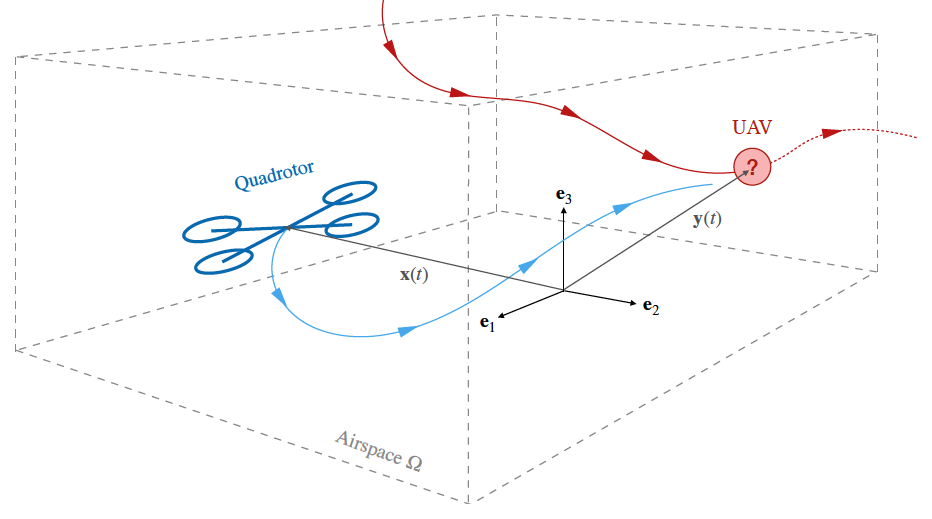
\includegraphics[width =0.45\textwidth]{images/ProjProbStmt.png}
%    \label{fig:prob}
%\end{figure}

\begin{multicols}{2}
\section*{Abstract}
The purpose of the project is to simulate the control and stable flight of an unmanned four rotor flying vehicle known as a quadrotor.  The problem is set into three goals: simulate and control the quadrotor hover in a stable configuration, chase an interloping quadrotor in flight and intercept, and return with the captured target quadrotor with randomized disturbance force while maintaining stable flight.

\section*{Introduction}
The mission is defense of a designated airspace.  Our quadrotor is assigned to monitor a limited airspace, launch if an unidentified 
UAV enters that airspace, capture the target, and return to base.  If the target leaves the airspace before being captured, our 
quadrotor should return to base.  When captured, the target should be assumed to generate external forces on our UAV.  Figure 1 of \cite{FaalP} depicts the scenario.
\section*{Methodology}
\textbf{General Approach}. We'll begin by generating the state space variables and defining the state space.  We'll prove 
controllability of the system and choose a controller methodology.  Using the controller, we will simulate hover as well as move to 
location and hover.  Finally we'll introduce external forces and moments that would be experienced simulating a target capture in the 
problem statement.  For ease of variable passing, our quadcopter will be represented as a structure in Matlab, with full state 
variables, A and B matrices, K gain matrix, $K_{capture}$ gain matrix (incorporating $n$ and $r$ forces and torques from the target) 
as well as characteristics for graphing (colors etc).

\noindent \textbf{Frames and Constants}. Coordinate frames are identified for the reference/inertial frame $E={e_1, e_2, e_3}$ at the center bottom of the airspace and the 
body frame $C={c_1, c_2, c_3}$.  All rotors are equidistant from the center of mass and in the same $c_1-c_2 $ plane as the body 
center of mass.  The external forces and moments on the system are represented by $\boldsymbol{r}$ and $\boldsymbol{n}$, where 
$\boldsymbol{r} = r_1 c_1 + r_2 c_2 + r_3 c_3$ and $\boldsymbol{n} = n_1 c_1 + n_2 c_2 + n_3 c_3$ directly applied to the center 
of mass. We are assuming that the torque of the rotor is proportionally related to the input thrust via the constant $\sigma>0$, for $
\tau_i = \sigma u_i$. We will be utilizing $\boldsymbol{I}$ as our diagonal inertial matrix where diagonal elements  $I_x, I_y $ and 
$I_z$ represent the mass moments of inertia about $c_1, c_2 $ and $c_3$ respectively.  For the purpose of our analysis we'll ignore 
the drag \textbf{and what other things}. The parameters for our state are described in Table 1 of \cite{FaalP} %

%$\ref{table:Qparams}$.
%\begin{table*} [htbp]%[t]
%\begin{centering}
%\begin{tabular}{|cccc|}
%\hline
%Parameter & Value & Units  & Description  \\
%\hline
% $l$  &  .02& m & Distance from center of mass to center of each rotor  \\
% $m$& .5 & kg &Total mass of quadrotor   \\
% $I_{x}$ & 1.24 kgm$^2 $ & s  & Mass moment of inertia about $c_1$ axis \\
% $I_{y}$ & 1.24 kgm$^2 $ & s  & Mass moment of inertia about $c_2$ axis \\
% $I_{z}$ & 1.24 kgm$^2 $ & s  & Mass moment of inertia about $c_3$ axis \\
%$ g$ &9.81 & m/s$^2$ & Gravitational acceleration\\
%$\sigma\ $& .01 & m & Proportionality constant relating $u_i $ to $\tau_i$\\
%\hline
%\end{tabular}
%\caption{Quadrotor Parameters}
%\label{table:Qparams}
%\end{centering}
%\end{table*}

\noindent \textbf{State Variable}.  Up to the state variable, development of the quadrotor equations are found in \cite{FaalD}.  We'll establish the state variable, $\mathbf{z}$ to represent the quadrotor's xyz 
center-of-mass position in the earth 
frame $\mathbf{x}=\begin{bmatrix}x_1 & x_2 & x_3\end{bmatrix}^T$; the roll, pitch, yaw angles in the earth frame, $\bm{\alpha}
=\begin{bmatrix}\phi & \theta & \psi\end{bmatrix}^T$; the xyz linear velocities in the earth frame, $\mathbf{v}=\begin{bmatrix}v_1 & 
v_2 & v_3\end{bmatrix}^T$; and the angular accelerations $\bm{\omega}=\begin{bmatrix}\omega_1 & \omega_2 & 
\omega_3\end{bmatrix}^T$ in the earth roll pitch yaw directions. Our state variable then is $\mathbf{z}=\begin{bmatrix}\mathbf{x}
&\bm{\alpha}&\mathbf{v}&\bm{\omega}\end{bmatrix}^T$. We define $\boldsymbol{\dot{z}}$ as $\begin{bmatrix} \mathbf{\dot{x}}
&\bm{\dot{\alpha}}&\mathbf{\dot{v}}&\bm{\dot{\omega}} \end{bmatrix}^T$, with:

\begin{equation}
    \mathbf{\dot{x}} =\mathbf{v}
\end{equation}
\begin{equation}
    \bm{\dot{\alpha}} =\mathbf{T}^{-1}\bm{\omega}
\end{equation}
\begin{align}
    \mathbf{\dot{v}} &=-ge_3+\frac{1}{m}\mathbf{R_{C/E}}(u_1+u_2+u_3+u_4)c_3 \nonumber\\ &+\frac{1}{m}\mathbf{R_{C/E}}r
\end{align}
\begin{align}
    \bm{\dot{\omega}} &=I^{-1}((u_2-u_4)lc_1+(u_3-u_1)lc_2 \nonumber\\ &+(u_1-u_2+u_3-u_4)\sigma c_3+n-\omega \times I \omega)
\end{align}

\noindent ...where $\mathbf{R_{C/E}}$ is defined in the problem statement as the Euler rotation matrix from quadrotor frame $C$ to earth frame $E$ and $\mathbf{T}^{-1}$, also defined in the problem statement, relates the angular rate of change of the Euler angles based on the angular velocity of the quadrotor.

Our system is nonlinear because it is under-actuated; four actuators for six degrees of freedom. We can utilize linearization to simplify this model and approximate its behaviour for easier control. To do this, we wish to approximate our system as $\boldsymbol{\dot{z}}=\boldsymbol{A}\boldsymbol{x}+\boldsymbol{B}\boldsymbol{u}$. We derive the $\boldsymbol{A}$ matrix as the Jacobian of our $\boldsymbol{\dot{z}}$ by $\boldsymbol{z}$, and our $\boldsymbol{B}$ as the Jacobian of our $\boldsymbol{\dot{z}}$ by $\boldsymbol{u}$. 

%Thus:
%\begin{equation}
%   \boldsymbol{A} = \begin{bmatrix}
%       \frac{\partial \dot{x}}{\partial x} &
%        \frac{\partial \dot{x}}{\partial y} &
%        \frac{\partial \dot{x}}{\partial z} &
%        \dots &
%        \frac{\partial \dot{x}}{\partial \omega_1} &
%        \frac{\partial \dot{x}}{\partial \omega_2} &
%        \frac{\partial \dot{x}}{\partial \omega_3}
%        \\[4pt]
%        \frac{\partial \dot{y}}{\partial x} &
%        \frac{\partial \dot{y}}{\partial \theta} &
%        \frac{\partial \dot{y}}{\partial \dot{x}} &
%        \dots &
%        \frac{\partial \dot{y}}{\partial \omega_1} &
%        \frac{\partial \dot{y}}{\partial \omega_2} &
%        \frac{\partial \dot{y}}{\partial \omega_3}
%        \\[4pt]
%        \vdots & \vdots & \vdots & \ddots & \vdots & \vdots & & \vdots
%        \\[4pt]
%        \frac{\partial \dot{\omega}_2}{\partial x} &
%        \frac{\partial \dot{\omega}_2}{\partial \theta} &
%        \frac{\partial \dot{\omega}_2}{\partial \dot{x}} &
%        \dots &
%        \frac{\partial \dot{\omega}_2}{\partial \omega_1} &
%        \frac{\partial \dot{\omega}_2}{\partial \omega_2} & 
%        \frac{\partial \dot{\omega}_2}{\partial \omega_3} 
%        \\[4pt]
%        \frac{\partial \dot{\omega}_3}{\partial x} &
%        \frac{\partial \dot{\omega}_3}{\partial \theta} &
%        \frac{\partial \dot{\omega}_3}{\partial \dot{x}} &
%        \dots &
%        \frac{\partial \dot{\omega}_3}{\partial \omega_1} &
%        \frac{\partial \dot{\omega}_3}{\partial \omega_2} &
%        \frac{\partial \dot{\omega}_3}{\partial \omega_3}
%    \end{bmatrix}
%\end{equation}

%\begin{equation}
%    \boldsymbol{B} = \begin{bmatrix}
%        \frac{\partial \dot{x}}{\partial u_1} &
%        \frac{\partial \dot{x}}{\partial u_2} &
%        \frac{\partial \dot{x}}{\partial u_3} &
%        \frac{\partial \dot{x}}{\partial u_4}
%        \\[4pt]
%        \frac{\partial \dot{y}}{\partial u_1} &
%        \frac{\partial \dot{y}}{\partial u_2} &
%        \frac{\partial \dot{y}}{\partial u_3} &
%        \frac{\partial \dot{y}}{\partial u_4}
%        \\[4pt]
%        \vdots & \vdots & \vdots & \vdots
%        \\[4pt]
%        \frac{\partial \dot{\omega}_2}{\partial u_1} &
%        \frac{\partial \dot{\omega}_2}{\partial u_2} &
%        \frac{\partial \dot{\omega}_2}{\partial u_3} &
%        \frac{\partial \dot{\omega}_2}{\partial u_4}
%        \\[4pt]
%        \frac{\partial \dot{\omega}_3}{\partial u_1} &
%        \frac{\partial \dot{\omega}_3}{\partial u_2} &
%        \frac{\partial \dot{\omega}_3}{\partial u_3} &
%        \frac{\partial \dot{\omega}_3}{\partial u_4}
%    \end{bmatrix}
%\end{equation}

For our approximation we model the quadrotor in a stable hovering position, where a given state is $\boldsymbol{z}=\begin{bmatrix} x & y & z & \boldsymbol{0}\end{bmatrix}^T$; no velocities, accelerations, and its orientation level. We assume a base output of $\frac{mg}{4}$, or each motor outputing the necessary force of a hover. We assign these values to our derived $\boldsymbol{A}$ and $\boldsymbol{B}$ matricies.

We wish to then confirm that our system is controllable with these matricies. We create a controllability matrix $\boldsymbol{C}$, which we define as $\boldsymbol{C} = \begin{bmatrix} A^0B & A^1B & A^2B & \dots & A^{n-3}B & A^{n-2}B & A^{n-1}\end{bmatrix}$ where $n$ is the size of our input, $12$. We must ensure that the combinations of our state and input matrices are linearly independent to the degree that we have an independent column for each state. To do so, we check rank of the controllability matrix $\boldsymbol{C}$ to assure that we have rank equal to the number of states in our z vector. As expected, the rank of our derived controllabiltiy matrix is indeed $12$.

We can utilize these to derive our $\boldsymbol{K}$ matrix to create a Linear-Quadratic Regulator (LQR) controller.

\section*{LQR Controller}
We selected the Linear-Quadratic Regulator (LQR) approach as an optimal control technique for generating the gain matrix, $
\boldsymbol{K}$.  LQR operates on our linearized system, utilizing both $\boldsymbol{A}$ and $\boldsymbol{B}$ matricies (states 
and inputs, respectively). LQR also utilizes two additional matrices- $\boldsymbol{Q}$ and $\boldsymbol{R}$, which correspond to $
\boldsymbol{A}$ and $\boldsymbol{B}$, respectively. $\boldsymbol{Q}$'s and $\boldsymbol{R}$'s purpose are to impose a weighted 
cost such that there will be trade off between particular elements of the state and inputs in the optimization. Since we are not asked 
to weigh the cost of using our actuators (as if we were conserving fuel), we have initially left both the  4x4 $\boldsymbol{R}$ matrix 
and 12x12 $\boldsymbol{Q}$ matrices as identity matrices, but found through experimentation that our 
desired performance required adjustments( to be discussed later in this paper). There is an additional matrix, $\boldsymbol{N}$, 
which acts as a penalty to the interactions between state variables and inputs.  We simplify by not using this.

LQR acts on the linearized system of the form $\dot{x} = Ax + Bu$ and calculates a cost function based on optimization.  This 
integrates the costs of both $\boldsymbol{Q}$ and $\boldsymbol{R}$ for comparison:
\begin{equation}
J =x_0^TF(0)x(t_0) +  \int_{t_0}^{t_f} x^TQx+u^TRu +2x^TNu\,dt 
\end{equation}

The control input u that minimizes this cost function is $u= -Kx$ with the K value is given by
\begin{equation}
K = R^{-1}(B^TP(t) + N^T)
\end{equation}
\noindent
Where P is created by solving Ricatti's continuous time differential equation:
\begin{align}
A^TP(t) + P(t)A - (P(t)B + N)R^{-1}(B^TP(t) + N^T) \nonumber\\+ Q = \dot{P}(t)
\end{align}
\noindent
and $P(t)$ is bounded by $P(0) = F(0)$. This process is repeated as we experimented with adjusting the weights within the $
\boldsymbol{Q}$ matrix.

Once we have our calculated $\boldsymbol{K}$, we define $z_d$ as the desired state of our quadrotor. If we are hovering at sending 
our quadrotor given point in space, it will be $z_d=\begin{bmatrix} x_{1_d} & x_{2_d} & x_{3_d} & \boldsymbol{0} 
\end{bmatrix}^T$. When we are chasing a given target through protected airspace, we will set the desired state to 
$z_d(t)=\begin{bmatrix} x_t(t) & \boldsymbol{0} \end{bmatrix}^T$ where $x_t(t)$ is the $x_1(t)$, $x_2(t)$, and $x_3(t)$ of the target at a given 
time $t$. We then calculate the error $e(t)$ as the difference between our desired state, or $z_d - z$. We utilize the error to 
determine the resulting inputs to our system, but we also must take note that since we assumed a linearized system around 
hovering, we must add an additional force of $\frac{mg}{4}$ to each of our input forces. Thus $\boldsymbol{u}= \boldsymbol{K}e(t) + 
\begin{bmatrix}\frac{mg}{4} & \frac{mg}{4} & \frac{mg}{4} & \frac{mg}{4}\end{bmatrix}$. 
Once we have calculated our $\boldsymbol{u}$, we limit the resulting outputs to to $u\  \epsilon\  (0, 3)$ as that is the max and 
minimum forces our motors can generate.
We then utilized the MATLAB ODE45 solver, utilizing our previously derived $\boldsymbol{\dot{z}}$ with calculated $
\boldsymbol{u}$. At each stage we determine what state of behavior we desire from our quadrotor - hover, move, and intercept - 
and from this determine the $z_d$. We then solve for our state variable $\boldsymbol{z}$ at each time increment.
\section*{Simulation}
\noindent
The foundation of simulating the controller is the solution of the system of differential equations of our original system with the added 
gain from our LQR controller.  We have wrapped the changes in the environment into a separate function to serve as the ODE 
function in order to incorporate time-related changes to the target path as well as n and r forces and torques after capture.\\
\textbf{Quadrotor Hovering.}. To demonstrate successful control of our quadrotor, we establish an initial state of $z=[\mathbf{0}]$ and 
a desired state $z_d=[5,5,5,0,0,0,0,0,0,0,0,0] $ to demonstrate move and hover.  Feeding these into our ODE45 solver, we obtain 
smooth movement and hovering at the given $z_d$.  (Note initial and final states as well as trajectory plotted) in Figure 1a.\\
\textbf{Quadrotor Return to Base}. A mission objective was to return to base if the target exits the envelope before capture.  
Figure 1b. demonstrates this performance. In this scenario the interceptor leaves the base to pursue the target, but the target exits 
the airspace envelope before the interceptor gets close enough to capture.\\
\textbf{Quadrotor Interception of Target}. For modeling we will input a piecewise continuous function for the target so that we can 
include it in a single differentiation.  In earlier iterations, we input random, continuous movements of the target which were only 
revealed to our quadcopter each second in a loop.  We resolved the ODE for new $z_d$ in that loop and were readily able to converge, so we believe the known "unknown" target trajectory to be an allowable simplification for solve time.
For interception, it is assumed that the target is intercepted if we get within a distance of .3m of it.   Our simulation demonstrates 
successful interception of the target after tuning the Q matrix to de-emphasize errors in the z direction (to enable smoother up/down 
movement) and penalize x-y errors.  \\
\textbf{Capture/RtB with Disturbance}.  For the disturbance forces and torques after capture,  in the control of the ODE function we trigger a change in $n$ and $r$ and re-evaluate K before adding the mass of the target drone to recalculate the control, $u$, term for the ODE.  Again we use the simplification of a time dependent function for the $n$ term $n=[\sin(t)/2; 0; 0]$ to simulate the target trying to escape.  Other $n$ vectors were also simulated.\\
\begin{figure}[H]
\centering
\begin{subfigure}[b]{0.45\columnwidth}
    \centering
    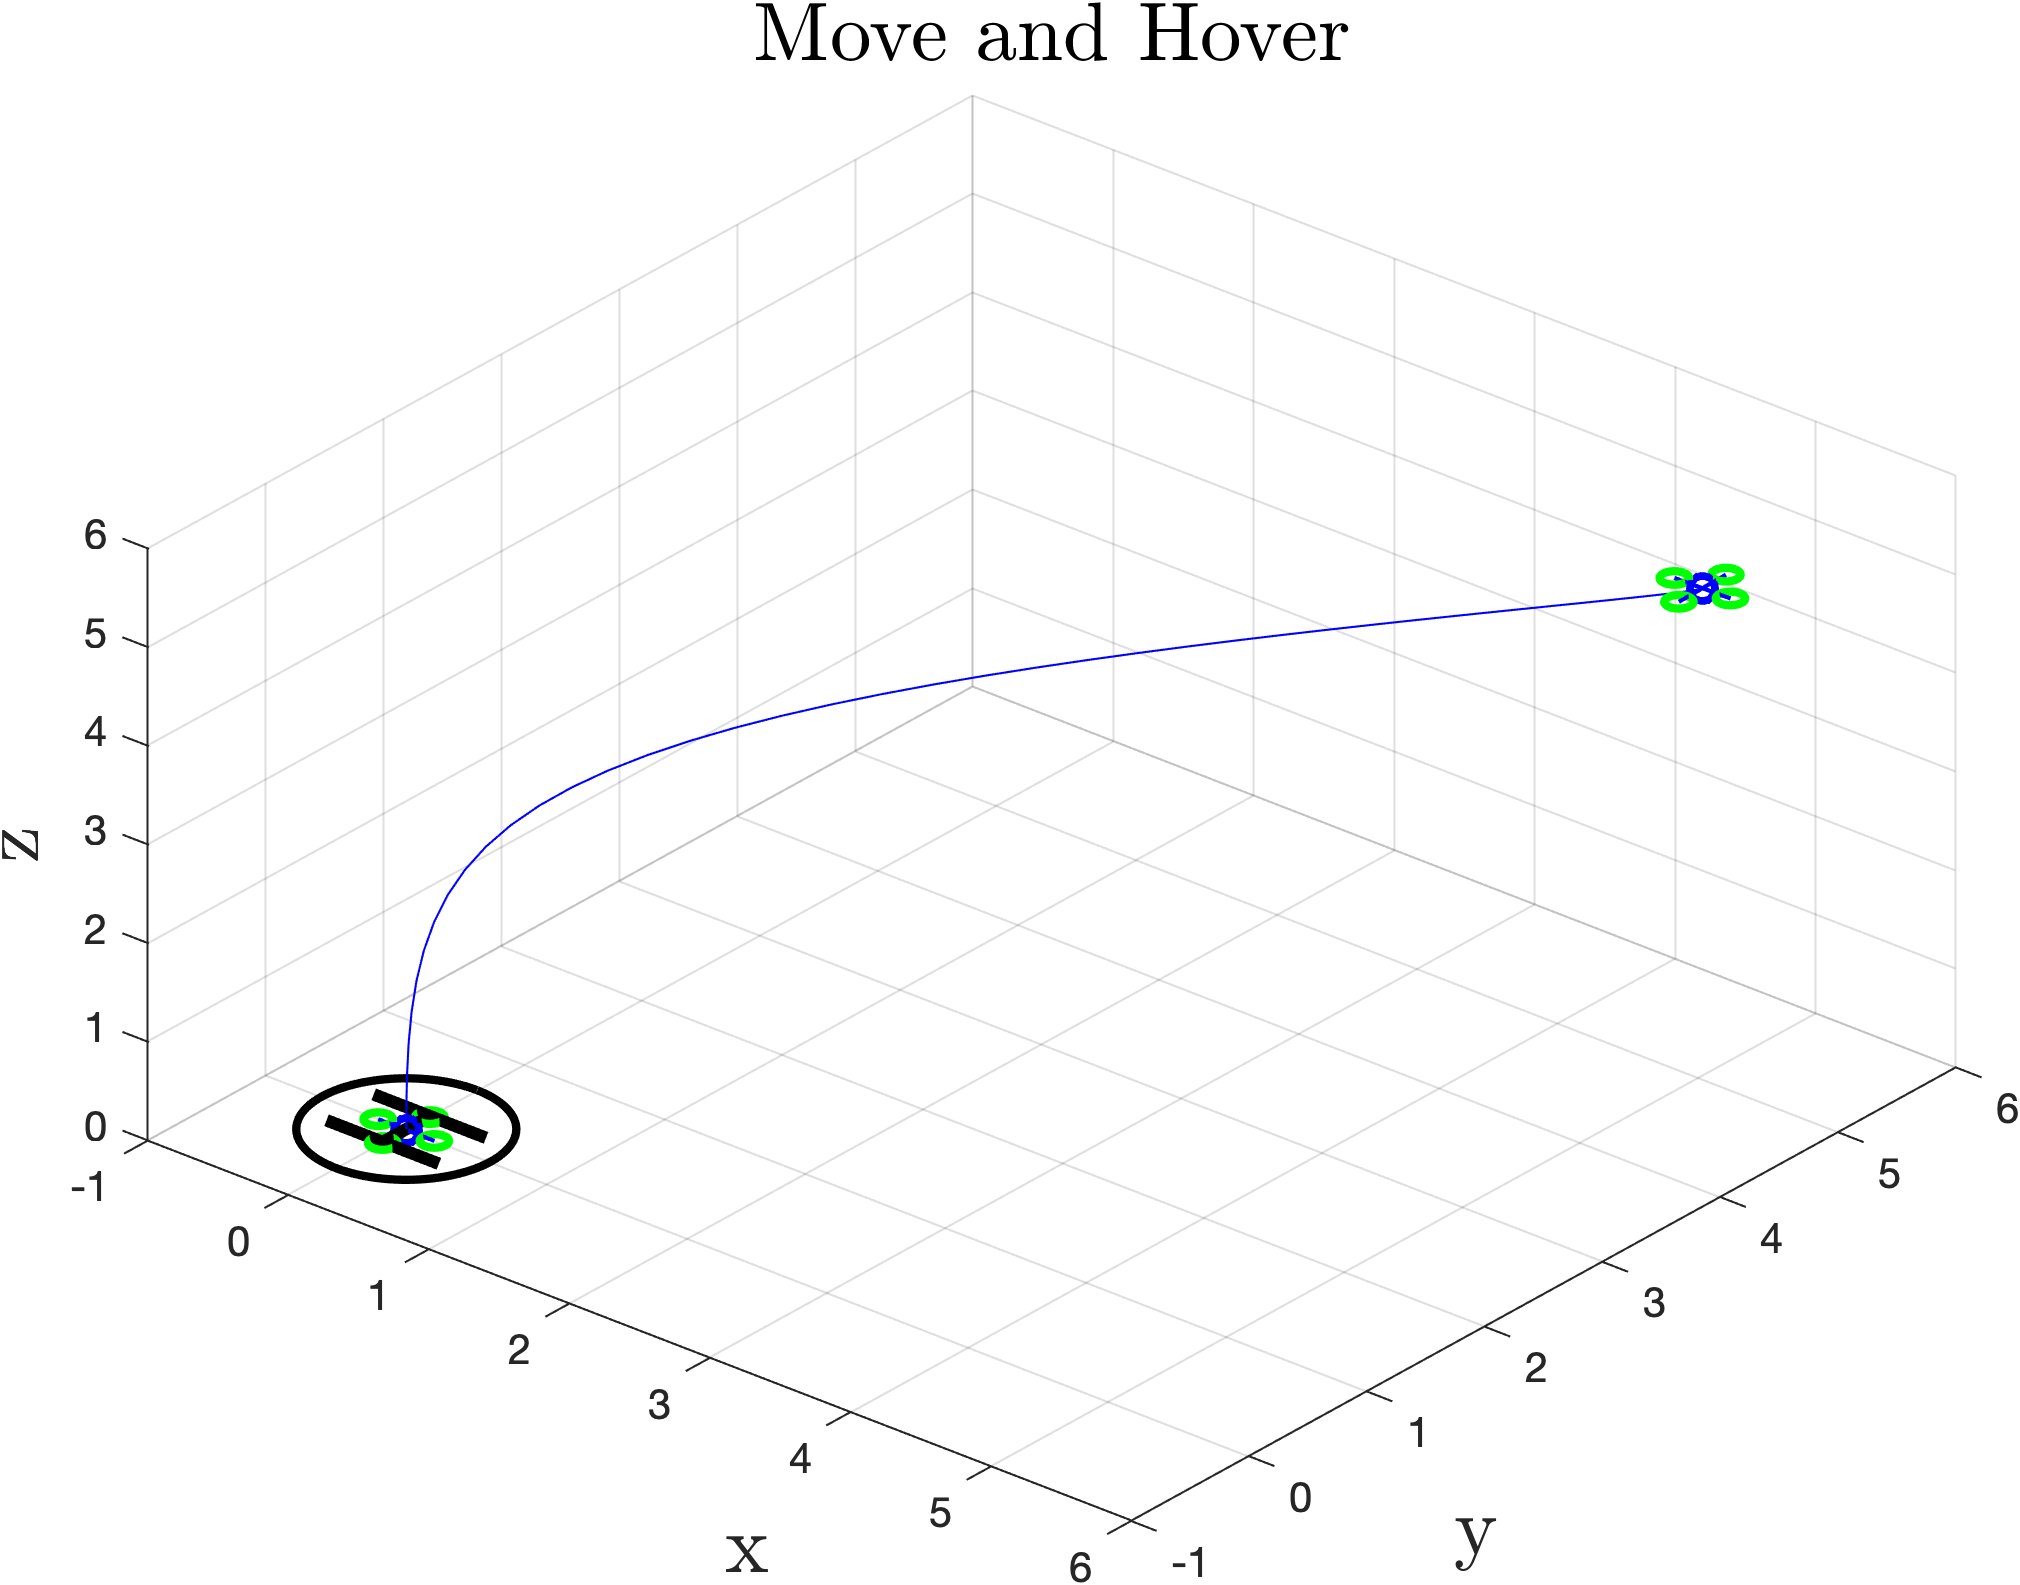
\includegraphics[width = 1\textwidth]{images/MoveAndHover.png}
     \label{fig:MandH}
     \vspace{-5mm}
     \caption{Move and Hover}
\end{subfigure}
\begin{subfigure}[b]{0.45\columnwidth}
    \centering
    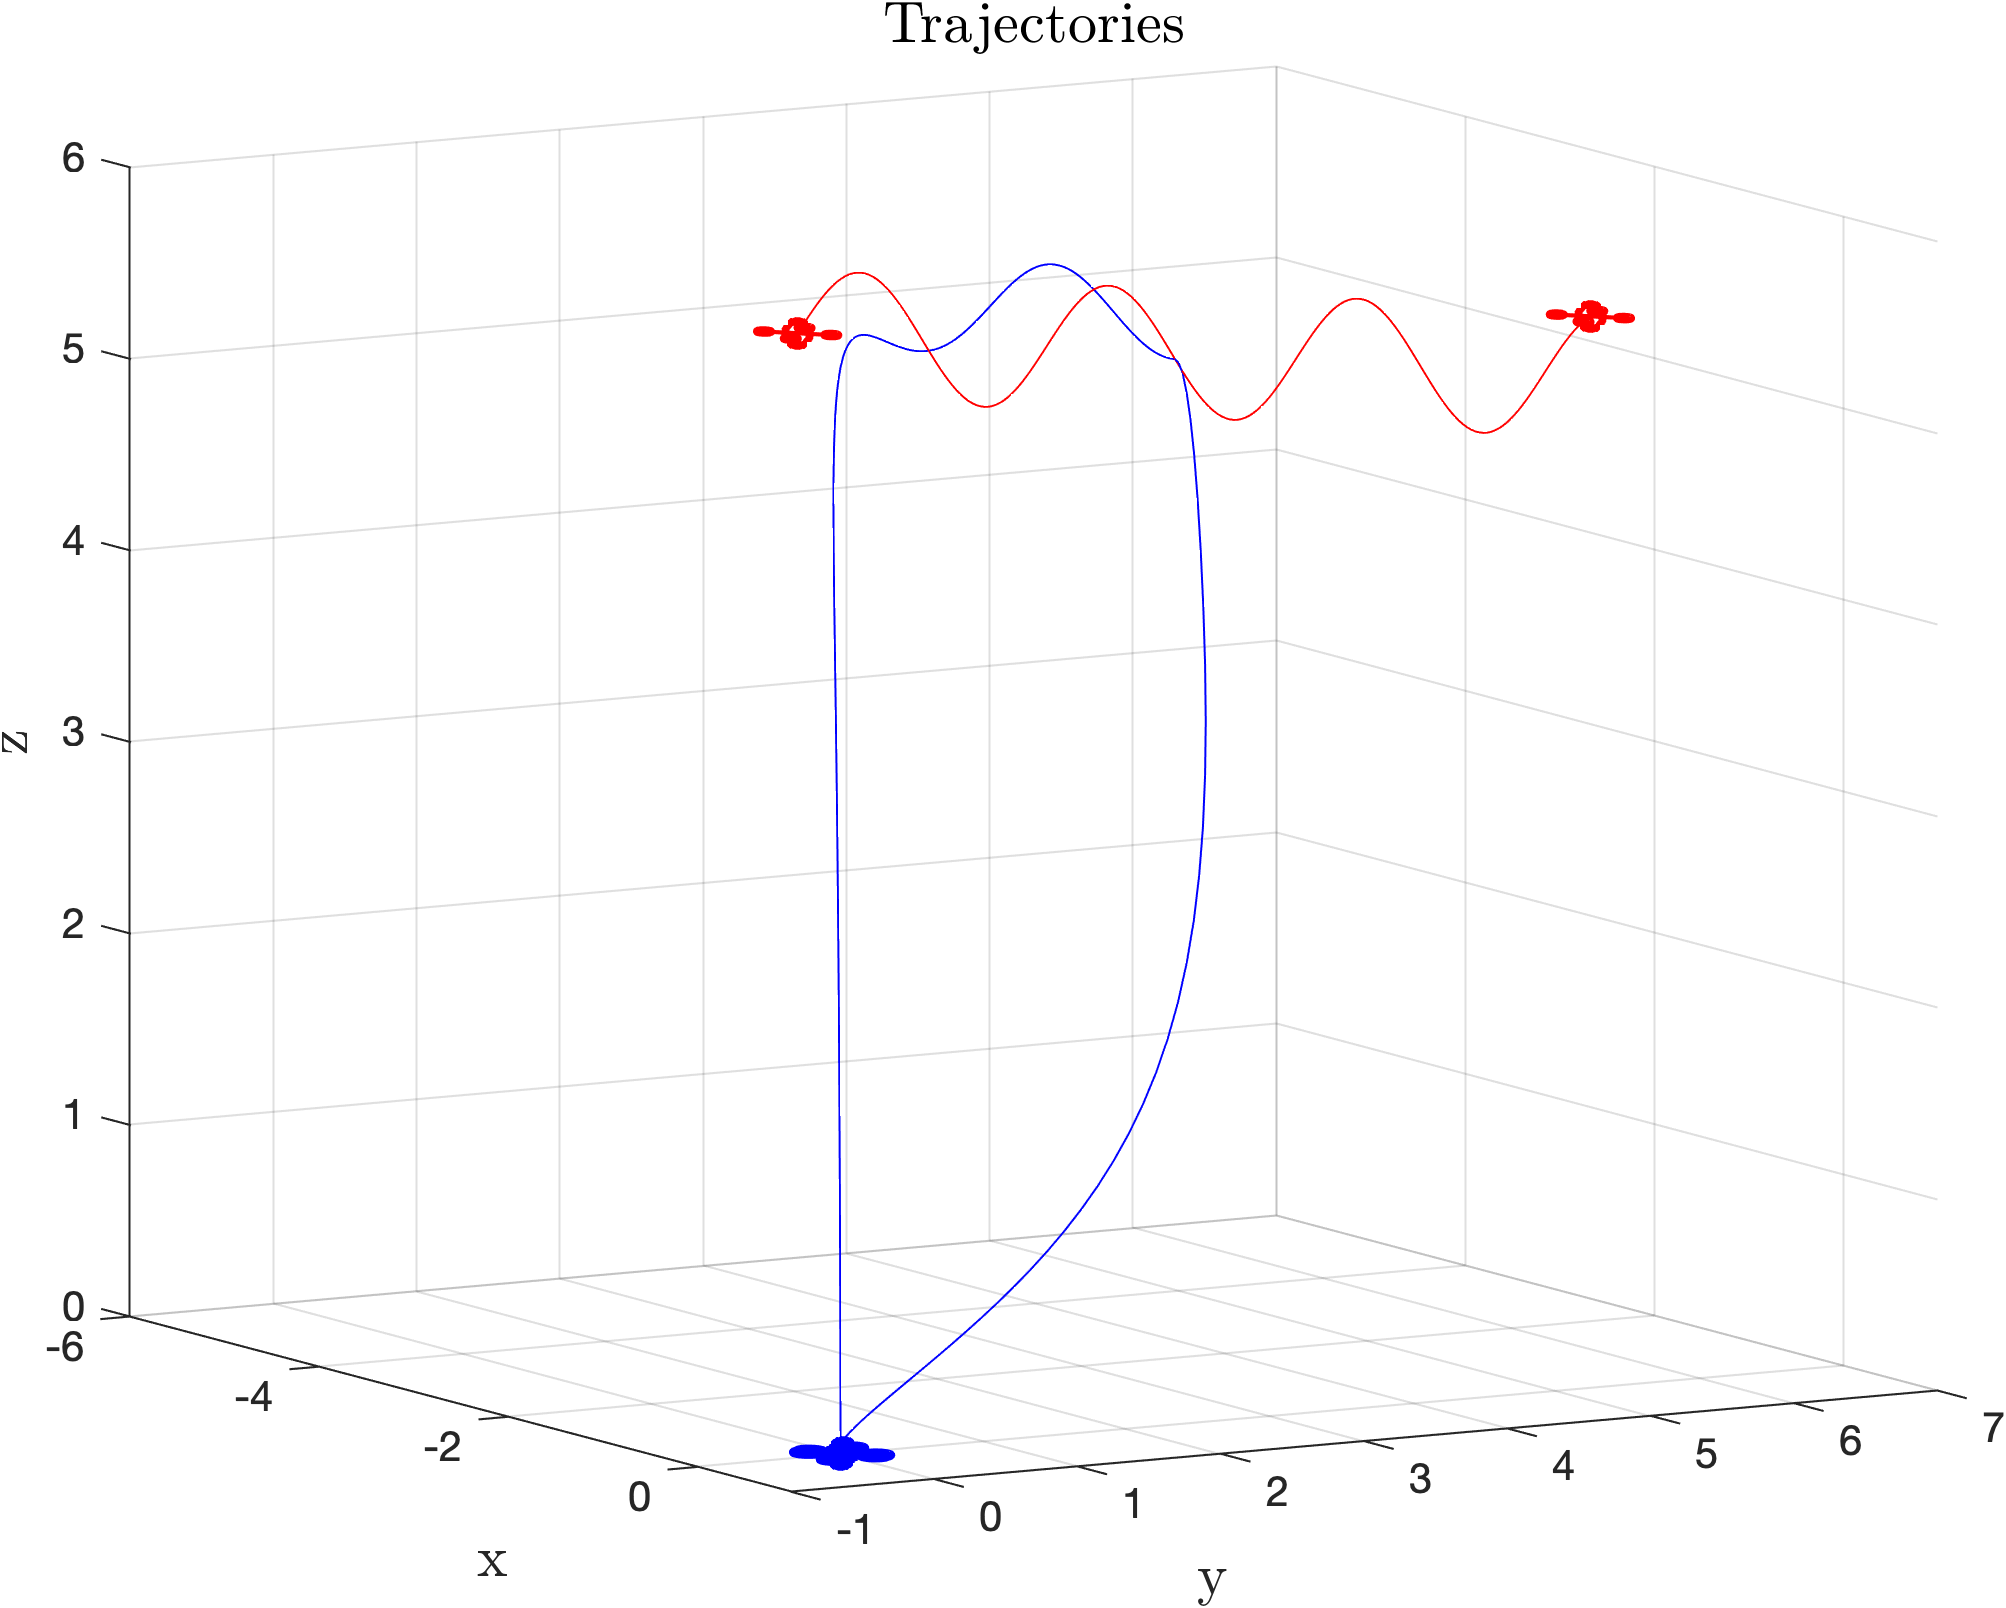
\includegraphics[width = 1\textwidth]{images/ReturnToBase.png}
     \label{fig:Return}
     \vspace{-5mm}
      \caption{Return to Base}
 \end{subfigure}
\begin{subfigure}[b]{0.45\columnwidth}
    \centering
    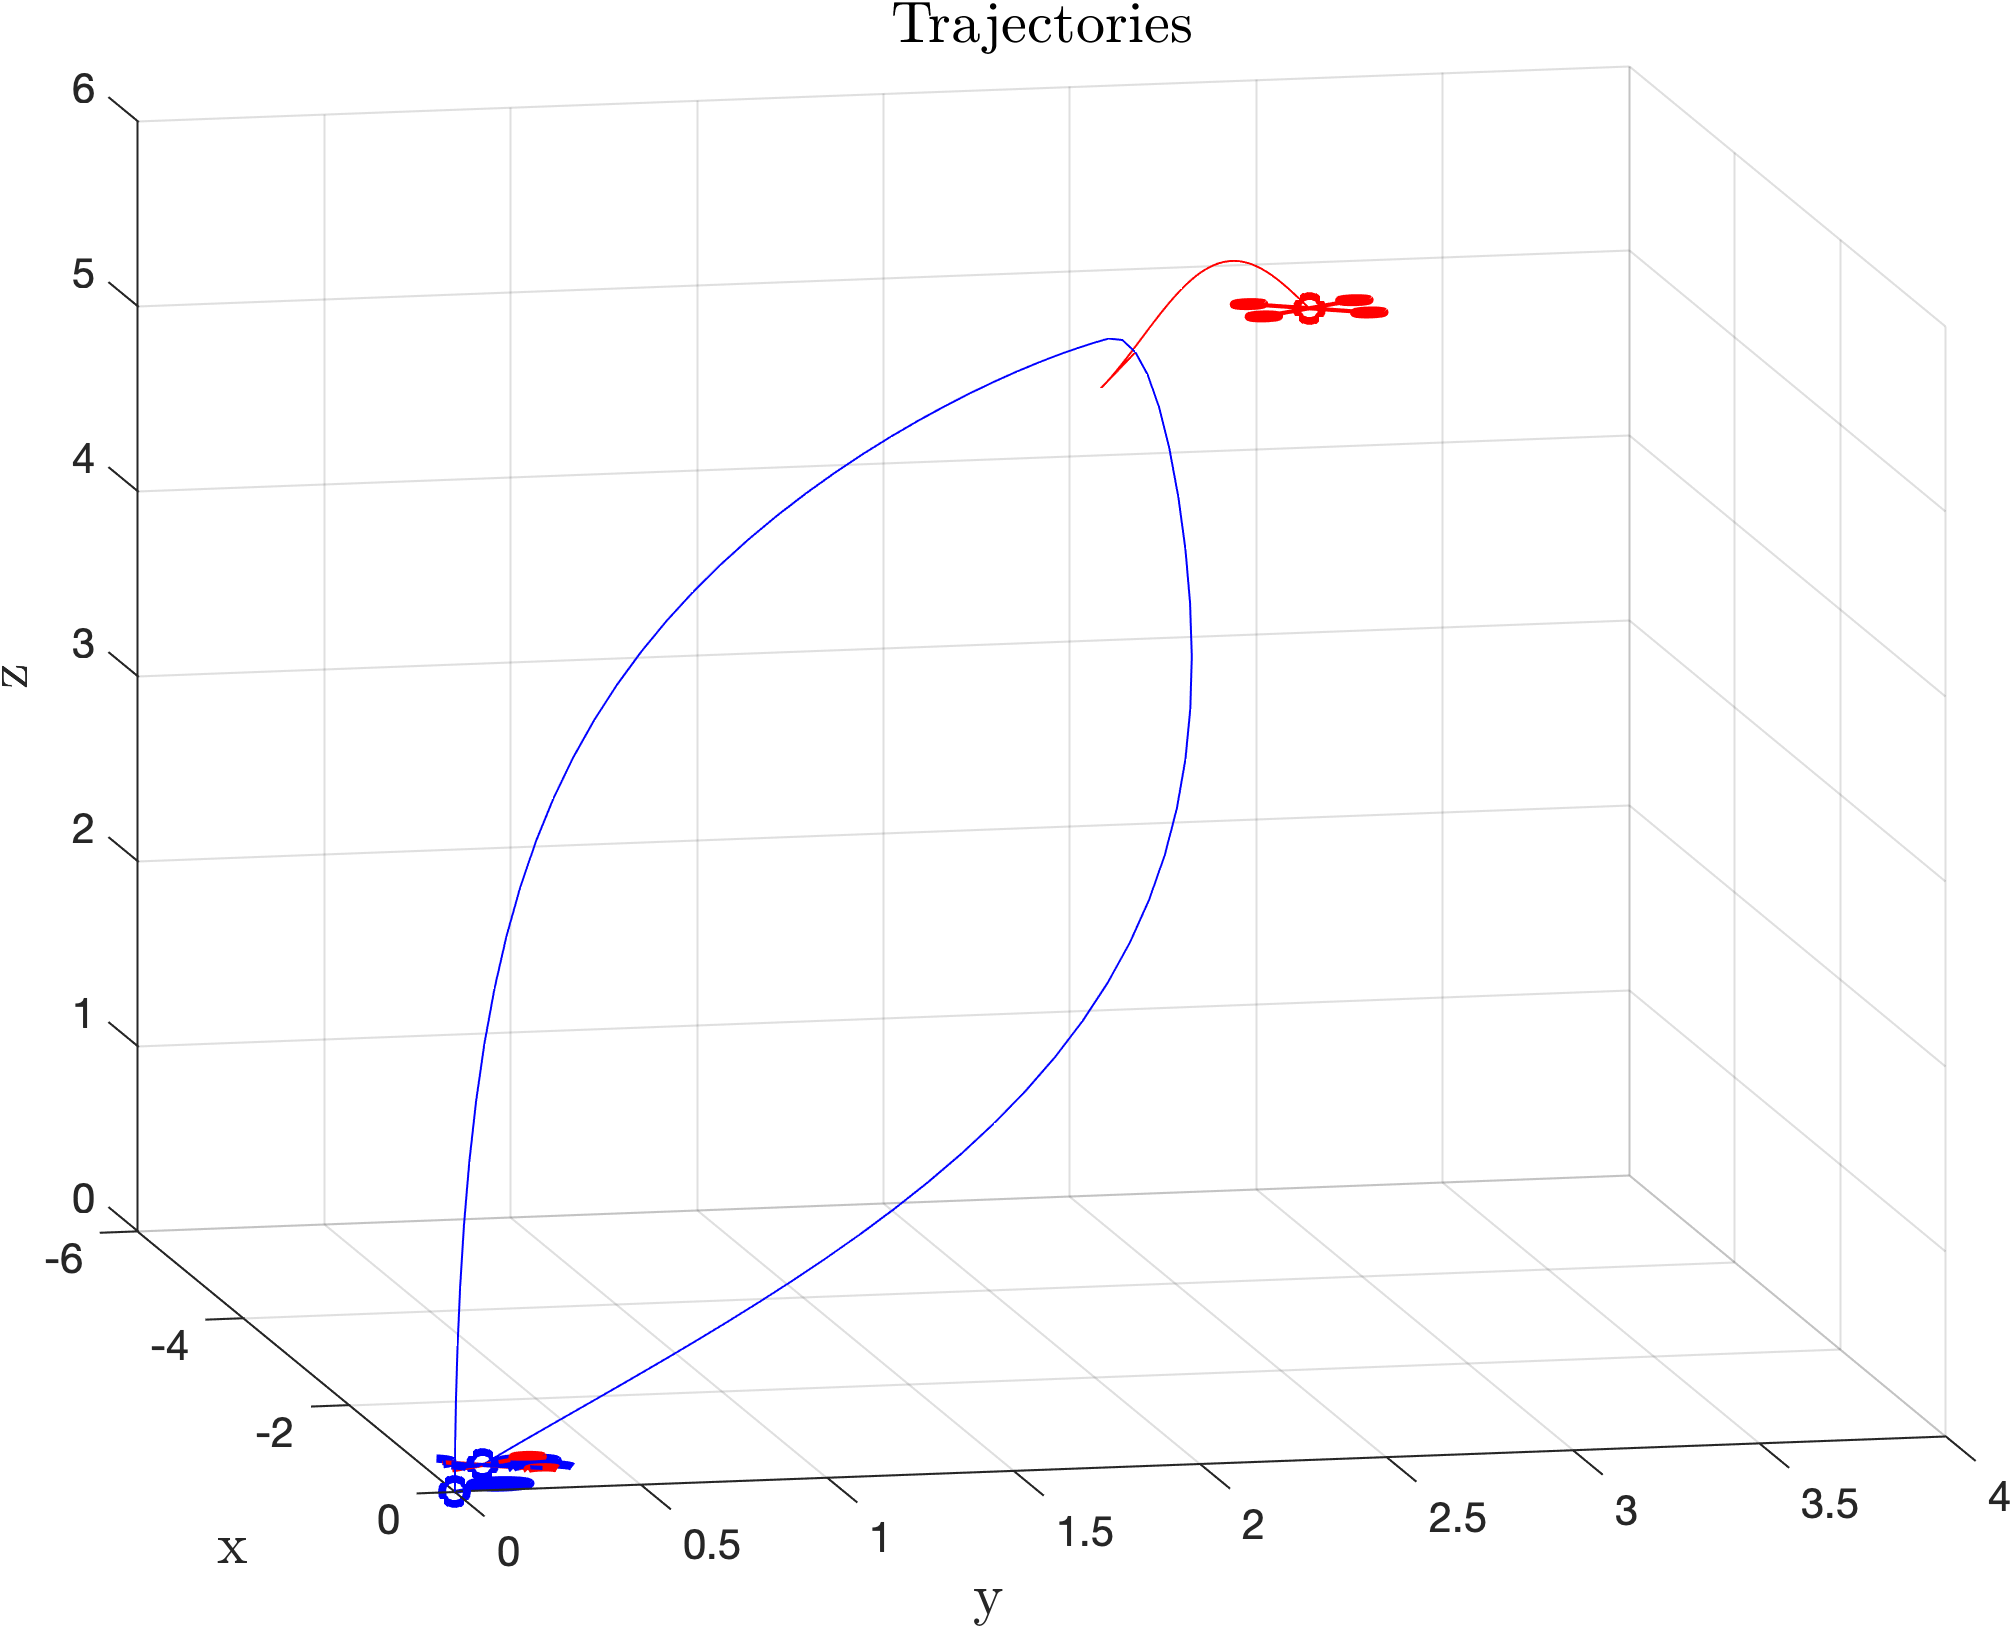
\includegraphics[width = 1\textwidth]{images/Intercept.png}
     \label{fig:Capture}
     \vspace{-5mm}
     \caption{Capture}
 \end{subfigure}
 \begin{subfigure}[b]{0.45\columnwidth}
    \centering
    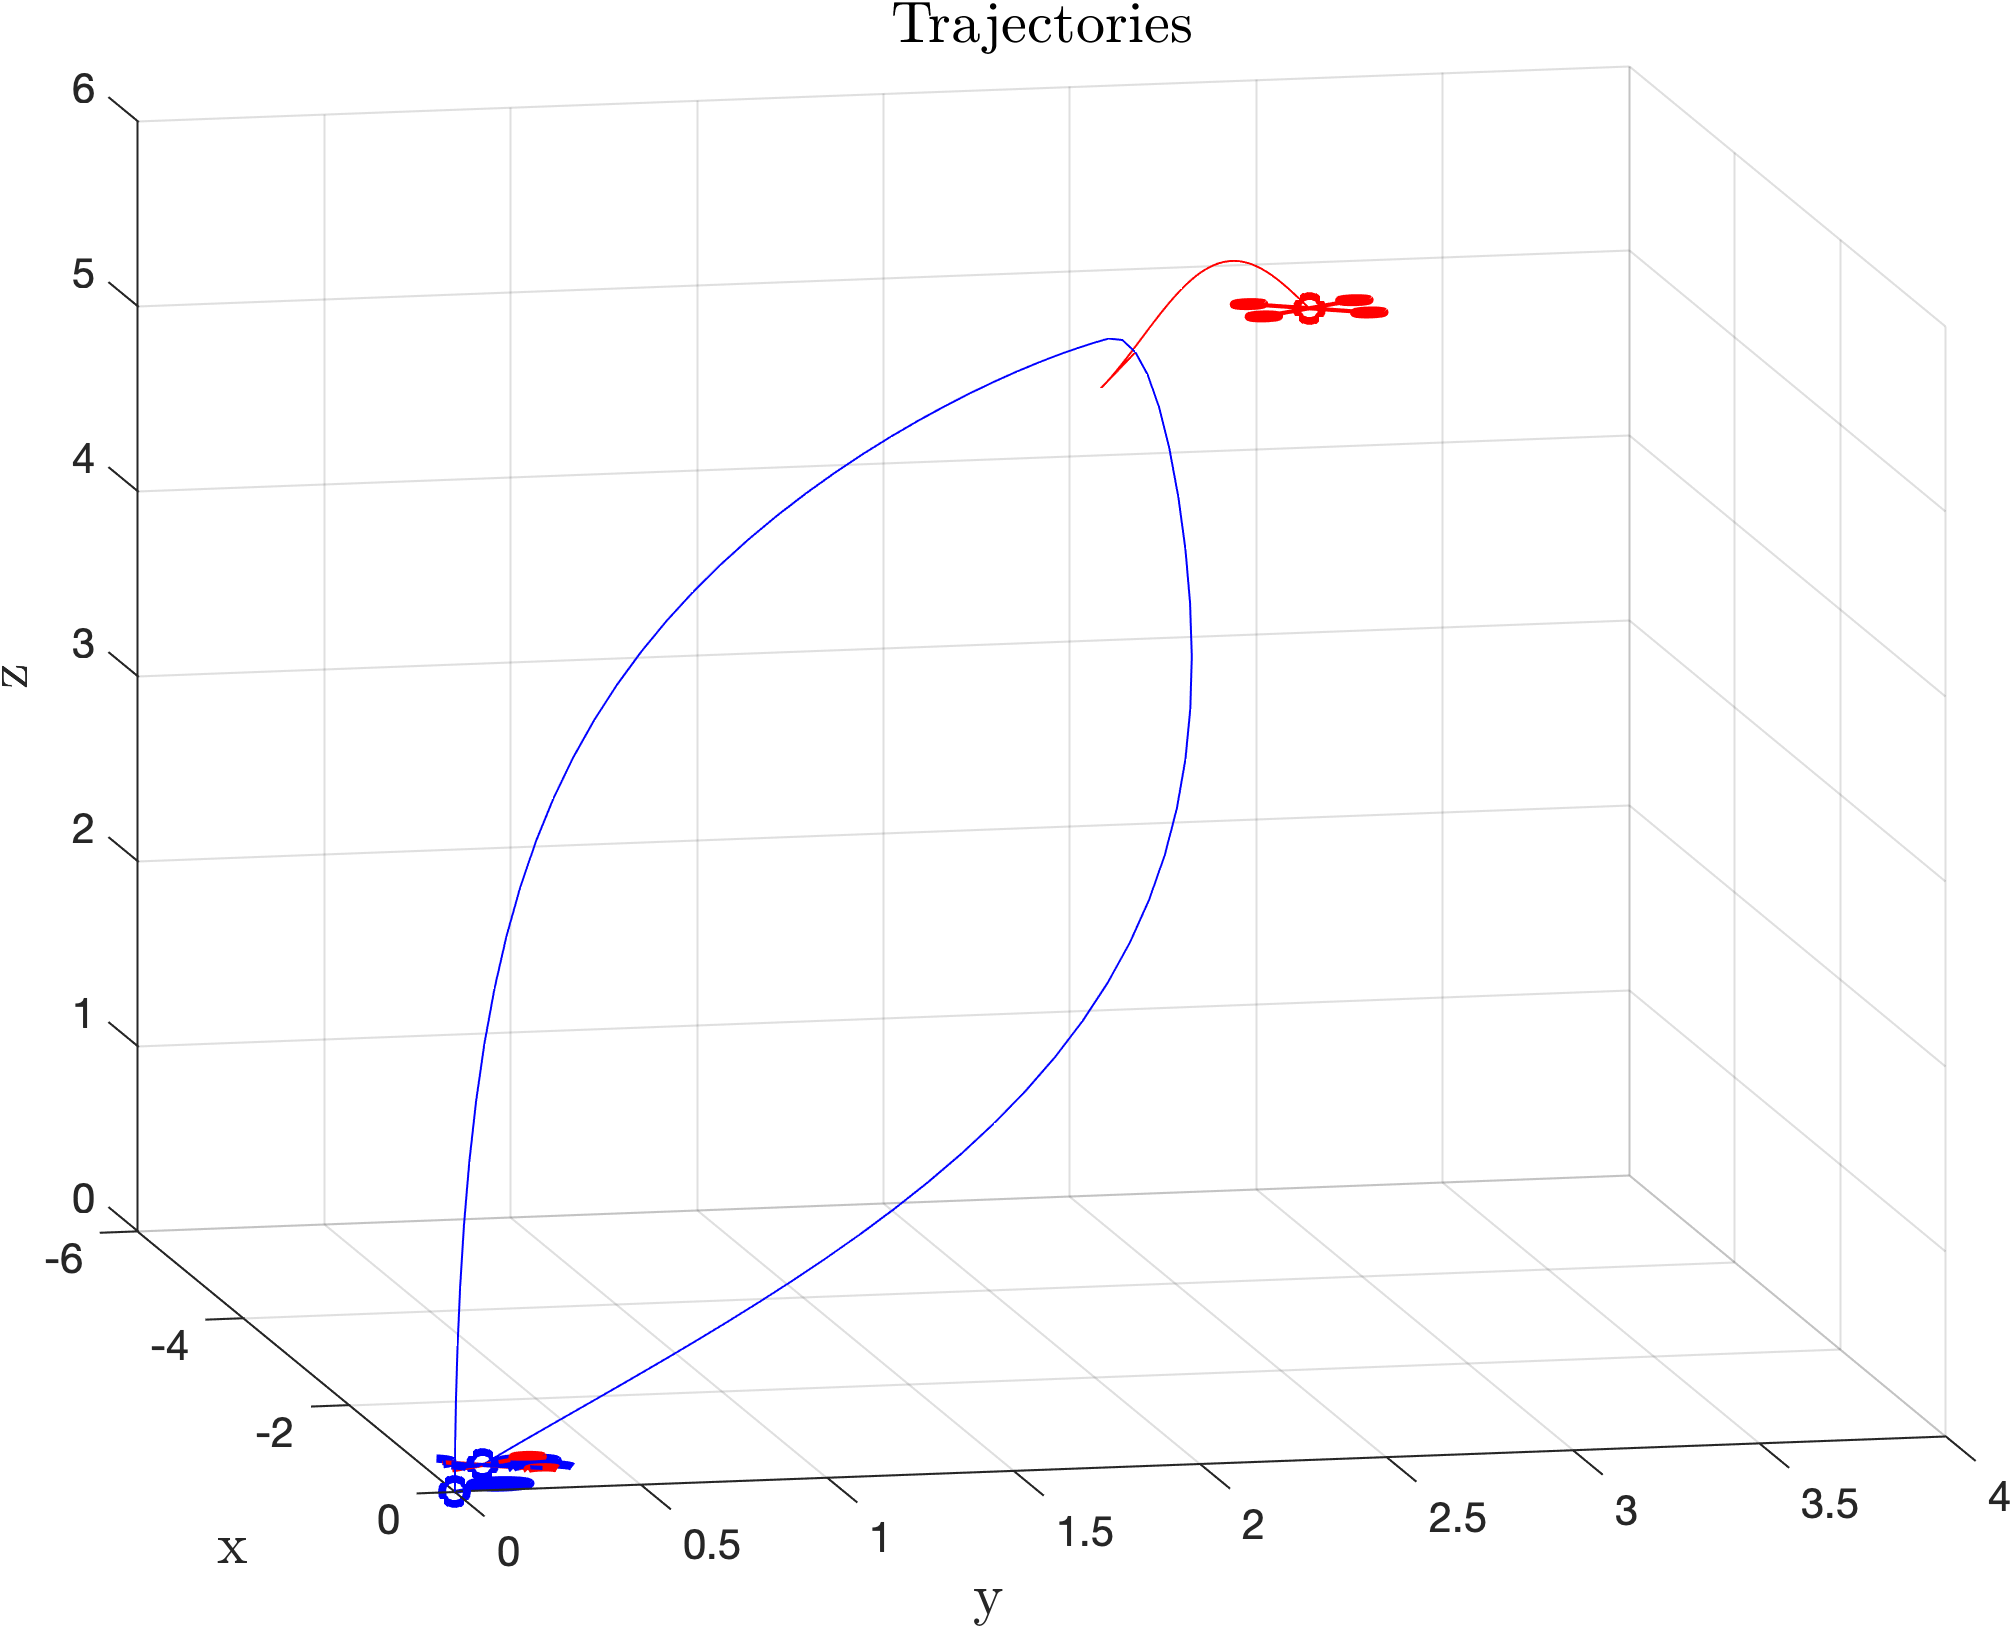
\includegraphics[width = 1\textwidth]{images/Intercept.png}
     \label{fig:CaptureW}
     \vspace{-5mm}
     \caption{Capture Disturbance}
 \end{subfigure}
   \caption{Quadrotor Performance Tests}
\end{figure}

\section*{Results}
We were unable to successfully return to base with a captured target given the limits (but this may not be the case if we fix A and B)?
\section*{Discussion}
Further research would tune the Q and R matrices.  Various external research suggests simply trial and error while other suggest optimization methods (blah-blah). A common method is to weight by the inverse of the maximum allowable error squared \cite{mur}.  We could also enhance the process to store target position to estimate the velocity vector to anticipate next target position.  This could improve time to intercept and allow use of Q weightings for velocity components. More advanced analysis could included power analysis to improve battery life of the quadrotor to extend mission life.
\label{References}
\bibliographystyle{abbrv}
\begin{thebibliography}{10}
\bibitem{JKim}
Jinho Kim, S. Andrew Gadsden, Stephen A . Wilkerson.
"A Comprehensive Survey of Control Strategies for Autonomus Quadrotors".
arXiv:2005.09858v1.
20 May 2020.
\bibitem{FaalP}
Faal, Siamak. Project Statement.  Class notes for RBE 502. Spring 2021.
\bibitem{FaalD}
Faal, Siamak. Notes on Control of Quadrotors. Class notes for RBE 502. March 3, 2021.
\bibitem{AHM}
Faraz Ahmad, Pushpendra Kumar, Anamika Bhandari, Pravin P. Patil.
Simulation of the Quadrotor Dynamics with LQR based Control.
Materials Today: Proceedings,Volume 24, Part 2, 2020, Pages 326-332,
ISSN 2214-7853.
https://doi.org/10.1016/j.matpr.2020.04.282.
\bibitem{OKY}
Okyere, E., Bousbaine, A., Poyi, G. T., Joseph, A. K., and Andrade.,
J. M. (2018) ‘LQR controller design for quad-rotor helicopters’,
The 9th International Conference on Power Electronics, Machines
and Drives. The Arena and Convention Centre, Liverpool, 17-19
April. London: The Institute of Engineering and Technology, pp.1-7
\bibitem{mur}
Murray, Richard M. Optimization Based Control.  California Institute of Technology. January 4th, 2010.
\bibitem{AHM}
\bibitem{MLT}



\end{thebibliography}

\end{multicols}

\end{document}

    © 2021 GitHub, Inc.
    Terms
    Privacy
    Security
    Status
    Docs

    Contact GitHub
    Pricing
    API
    Training
    Blog
    About

